\providecommand{\main}{../../..}
\documentclass[\main/main.tex]{subfiles}
\begin{document}

\subsection{Exercise 11}
The following problem is given:

\begin{align*}
  \min f_1\rnd{x} = x^2 - 4x \\
  \min f_2(x) = -x^2         \\
  x & \geq 0                 \\
  x & \leq 3                 \\
\end{align*}


Represent the utopy point $U$ in the space of the objectives and identify which one of the impacts $A' = (-4, -4)$ and $B' = (-3, -9)$ is preferable according to the euclidean distance from $U$.

Add another objective $f_3 = x$, always to minimize, and identify the values for which the relative weight $\w_3$ the point $x = 3$ constitutes the optimal solution, considering $\w_1 = \w_2$.

\subsection{Resolution exercise 11}
The minimum value the objectives can reach is, in the given domain, respectively $-4$ and $-9$, so the utopy point is $U = (-4, -9)$.

The euclidean distance from the points $A'$ and $B'$ is $5$ and $1$ respectively, so $B'$ is preferable.

If the weights $\w_1 = \w_2 \Rightarrow \w_1 = \frac{1 - \w_3}{2}$. Therefore, the objective function is:

\[
  f^* = \frac{1 - \w_3}{2}(x^2+4x) - \frac{1 - \w_3}{2}x^2 + \w_3 x = 2(1 - \w_3)x + \w_3x = 2x - \w_3x
\]

The range is obtainable by replacing $x=3$ in the function and resolving the following inequality:

\begin{align*}
  6 - 3\w_3 & \geq 2x - \w_3x \quad \forall x \in [0,3] \\
  6 - 2x    & \geq (3-x)\w_3                            \\
  \w_3      & \leq \frac{6-2x}{3-x} = 2
\end{align*}

Since the maximum value of $\w_3$ is $1$, there is no value for which $x = 3$ isn't an optimal solution.

Let's verify graphically:

\begin{figure}
  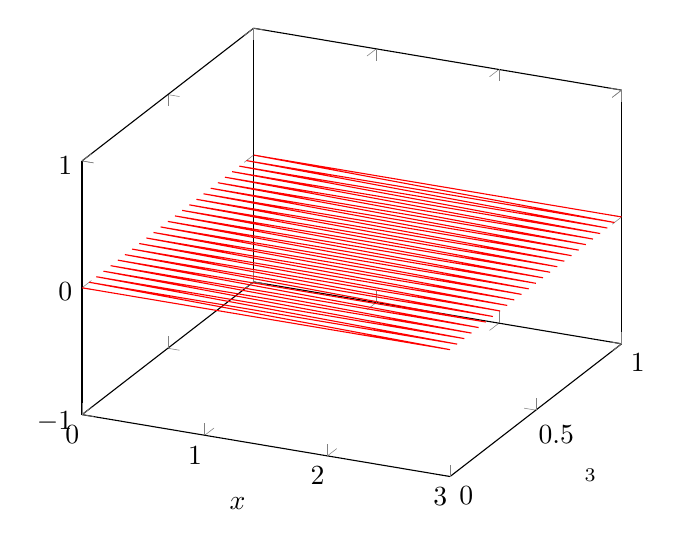
\begin{tikzpicture}
    \begin{axis}[
        xlabel=$x$,
        ylabel=$\w_3$,
        domain=0:3,
        y domain=0:1
      ]

      \addplot3[mark=none,color=red]{6-3*y >= 2*x - y*x?0:NaN};

    \end{axis}
  \end{tikzpicture}

\end{figure}

\end{document}